\usepackage{etex} %эта магическая херь избавляет от переполнения регистров TeX а!!!

\mode<article>{\usepackage{fullpage}}
\mode<presentation>{
    \usetheme{Madrid}
    \useoutertheme{shadow}
} 

\usepackage[utf8]{inputenc}
\usepackage[russian]{babel}
\usepackage{indentfirst}
\usepackage{graphicx}

\usepackage{amsmath}
\usepackage{amsfonts}
\usepackage{amsthm}
%\usepackage{algorithm}
%\usepackage{algorithmic}

%\usepackage[all]{xy}

\date{Лекция по дисциплине <<методы и средства защиты компьютерной информации>> (\today)}
\author[М.~М.~Шихов]{Михаил Шихов \\ \texttt{\underline{m.m.shihov@gmail.com}}}

%%для рисования графов пакетом xy-pic
%\entrymodifiers={++[o][F-]}

%%для псевдокода алгоритмов (algorithm,algorithmic)
%\renewcommand{\algorithmicrequire}{\textbf{Вход:}}
%\renewcommand{\algorithmicensure}{\textbf{Выход:}}
%\renewcommand{\algorithmiccomment}[1]{// #1}
%\floatname{algorithm}{Псевдокод}

%\setbeamercolor{alerted text}{fg=-green} %gyan, blue, green, -green

\title[Аппаратный ключ]{Методы аутентификации.\\Аппаратно-программный ключ.\\Признак <<что имеет>>}


\begin{document}


%титул и содержание статьи
\mode<article>{\maketitle\tableofcontents}

%титул и содержание презентации
\frame<presentation>{\titlepage}
\begin{frame}<presentation>
    \frametitle{Содержание}
    \tableofcontents
\end{frame}


\section{Аутентификация}


\subsection{Основы}


\begin{frame}
\frametitle{Аутентификация}
    \begin{definition}%theorem, lemma, proof, corollary, example
        \alert{Аутентификация} --- это проверка подлинности
    \end{definition}
    Аутентификация может быть произведена на основе проверки следующих признаков.
    \begin{enumerate}
        \item Something you know (Что знает).
        \item \alert{Something you have (Что имеет)}.
        \item Something you are (Чем является).
        \item Something you can (Что умеет).
    \end{enumerate}
\end{frame}


\begin{frame}
\frametitle{Аутентичность}
Возникает необходимость в аутентификации всех компонент информационной системы:
\begin{itemize}
    \item персонала;
    \item клиентов (их автоматизированных систем);
    \item поставшиков (их автоматизированных систем);
    \item программных и программно-аппаратных средств;
    \item данных.
\end{itemize}
В данном случае, аутентификации подлежит как человек, так и программное обеспечение.
\end{frame}


\section{Аппаратно-программный ключ}


\subsection{Области применения}


\begin{frame}
\frametitle{Области применения}
\begin{itemize}
    \item Аутентификация пользователя в ИС.
    
    \item Контроль физического доступа.
    
    \item Идентификация.\mode<article>{Например, домашних животных. Получают развитие идеи <<электронного>> паспорта.}
    
    \item Защищенное хранение данных.
    \begin{itemize}
        \item Cекретных ключей.
        \item Идентификации (например, паспортных).
        \item Биометрических.
    \end{itemize}
    
    \item Генерация секретных данных (ключей).
    
    \item Защита программного обеспечения и данных от нелегального.
    \begin{itemize}
        \item Копирования.
        \item Распространения.
        \item Использования.
    \end{itemize}
\end{itemize}
\end{frame}


\subsection{Варианты исполнения}


\begin{frame}
\frametitle{Варианты исполнения}
\begin{itemize}
    \item Ключи на базе iButton.
    
    \item Радиочастотные метки (RFID\footnote{Radio Frequency IDentification}).
    
    \item Контактные и бесконтактные смарт-карты\footnote{Также чип-карты. Карты с программно-аппаратным обеспечением.}.
    
    \item USB-ключи.
\end{itemize}
\end{frame}


\section{Устройства}


\subsection{iButton}


\begin{frame}
    \frametitle{Ключи на базе iButton}
    \framesubtitle{Внешний вид}
    
    \begin{figure}
        \begin{center}
            \mode<presentation>{ 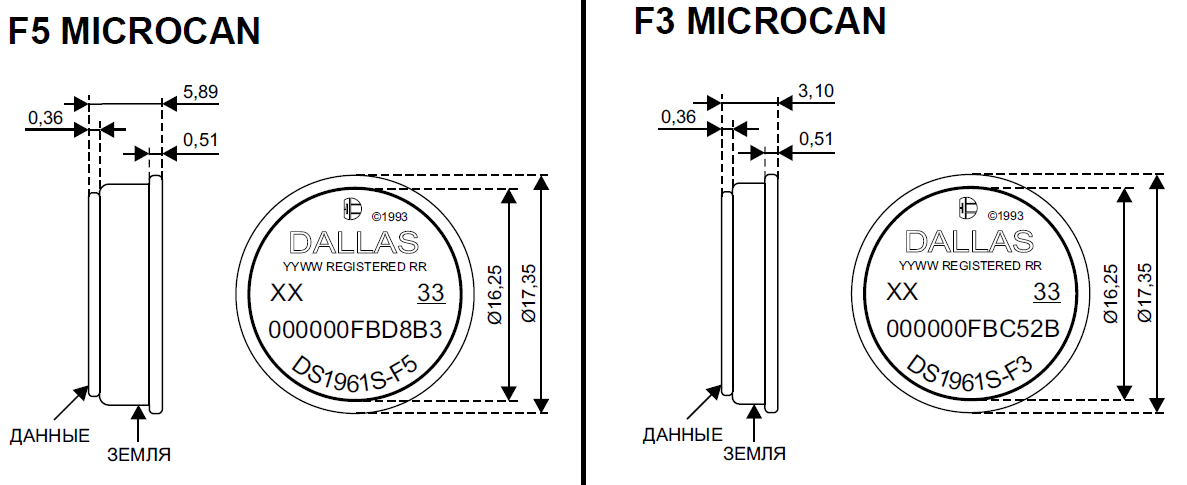
\includegraphics[width=.7\textwidth]{pict/ibutton} }
            \mode<article>{ 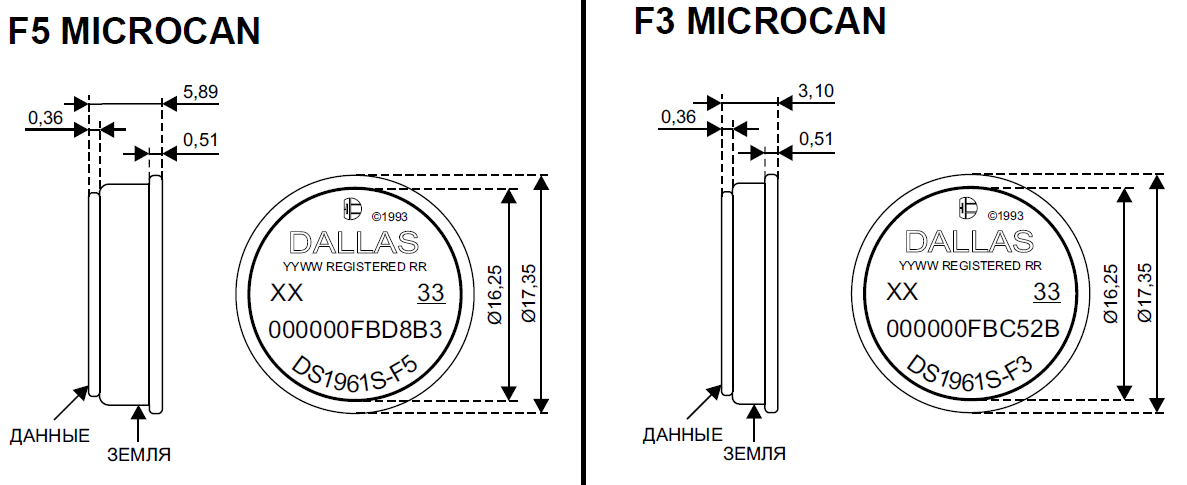
\includegraphics[width=.7\textwidth]{pict/ibutton} } 
            \caption{Таблетка iButton (размеры в мм.)}\label{pict:ibutton}
        \end{center}
    \end{figure} 
    
    \mode<article>{см. Рис. \ref{pict:ibutton}}
\end{frame}


\begin{frame}
    \frametitle{Ключи на базе iButton}
    \framesubtitle{Области применения}

    \begin{itemize}
        \item Системы контроля физического доступа (DS1990A --- простейший ключ).
            \mode<article>{
                Считывается 64 бита, 48 бит --- уникальный серийный номер, 
                8 бит --- тип идентификатора, 8 бит --- контрольная сумма.
            }
        \item Температурный мониторинг (сельское хозяйство).
        \item Контроль и учет (идентификация единиц хранения,счетчики тепловой энергии,
            временной мониторинг,санатории и лечебные учреждения,контроль патрульных служб,детектор событий).
        \item Средство проведения электронных платежей (платежи на общественном транспорте,средство 
            доставки электронных квитанций).
    \end{itemize}
\end{frame}


\begin{frame}
\frametitle{Ключи на базе iButton}
\framesubtitle{Особенности}
\begin{itemize}
    \item Интерфейс: 1-wire (16/142 KiBit/sec). Два типоразмера.
    \item Надежность(прочный корпус, защита от ЭМИ).
    \item Время хранения информации не менее 10 лет.
    \item Невысокая стоимость.
    \item Возможность использования в автономном режиме.
        \mode<article>{Например,установка таблеток на трубопроводах в автономном режиме (DS1994)}
    \item Возможность организовать сеть на основе 1-wire.
    \item Поддержка безопасности.
    \begin{itemize}
        \item Память с парольной защитой (DS1977,DS1991)
        \item Электронный кошелек. Поддержка SHA-1. (DS1961S,DS1963)
        \item Криптопроцессор. Поддержка Java Card 2.0. (DS1955B,DS1957B)
    \end{itemize}
\end{itemize}
\end{frame}


\subsection{RFID}


\begin{frame}
    \frametitle{RFID. Радиочастотные метки}
    \framesubtitle{Внешний вид}
    
    \begin{figure}
        \begin{center}
            \mode<presentation>{ \includegraphics[width=.4\textwidth]{pict/rfid} }
            \mode<article>{ \includegraphics[width=.4\textwidth]{pict/rfid} } 
            \caption{RFID --- метка}\label{pict:rfid}
        \end{center}
    \end{figure} 
    
    \mode<article>{см. Рис. \ref{pict:rfid}}
\end{frame}


\begin{frame}
    \frametitle{RFID. Радиочастотные метки}
    \framesubtitle{Области применения}
    
    RFID применяются преимущественно с целью идентификации.
    \begin{itemize}
        \item Промышленность, сельское хозяйство, транспорт.
        \item Управление товарами.
        \item Логистика.
        \item Системы контроля физического доступа.
        \item Медицина.
        \item Библиотечное дело.
        \item Паспорта.
        \item Опознавание животных.
        \item Локализации объектов в реальном режиме времени.
    \end{itemize} 
\end{frame}


\begin{frame}
\frametitle{RFID. Радиочастотные метки}
\framesubtitle{Особенности}
\begin{itemize}
    \item Низкочастотные (30-300 кГц) с дальностью (<1 см.); Высокочастотные (3-30 МГц) с дальностью (<1 м.); Сверхвысокочастотные (300 МГц--5.8 ГГц) с дальностью (>1 см.).
    \item Обеспечение энергией.
    \begin{itemize}
        \item Пассивные не имеют собственного источника питания и 
            получают энергию от электромагнитного сигнала от считывателя.
        \item Активные имеют собственный источник питания.
    \end{itemize}
    \item Запись информации.
    \begin{itemize}
        \item Read Only. Только чтение. Данные записываются изготовителем.
        \item WORM (Write Once Read Many). Пользователь может один раз записать информацию, 
            которая затем может быть считана неоднократно.
        \item R/W. Многократное чтение и запись.
    \end{itemize}
\end{itemize}
\end{frame}
\begin{frame}


\frametitle{RFID. Радиочастотные метки}
\framesubtitle{Стандарты}
\begin{itemize}
    \item RFID для управления товарами (RFID for item management).
    \begin{itemize}
        \item ISO/IEC:15961,15962,15963; ISO/IEC 18000-[1-7]; ISO/IEC TR 24729-[1-2].
    \end{itemize}
    
    \item Идентификация животных (Radio frequency identification of animals).
    \begin{itemize}
        \item ISO:24631-[1-4]; ISO:14223-[1-2]:2010; ISO 11784; ISO 11785.
    \end{itemize}
\end{itemize}
\end{frame}


\subsection{Чип-карты}


\begin{frame}
    \frametitle{Чип-карты}
    \framesubtitle{Внешний вид}
    
    \begin{figure}
        \begin{center}
            \mode<presentation>{ 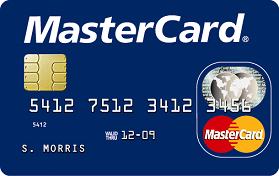
\includegraphics[width=.4\textwidth]{pict/card} }
            \mode<article>{ 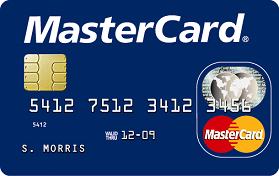
\includegraphics[width=.4\textwidth]{pict/card} } 
            
            \mode<presentation>{ 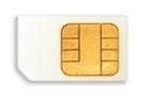
\includegraphics[width=.2\textwidth]{pict/chcard} }
            \mode<article>{ 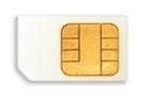
\includegraphics[width=.2\textwidth]{pict/chcard} } 
            
            \caption{Чип-карты}\label{pict:card}
        \end{center}
    \end{figure} 
    
    \mode<article>{см. Рис. \ref{pict:card}}
\end{frame}


\begin{frame}
    \frametitle{Чип-карты}
    \framesubtitle{Области применения}
    
    \begin{itemize}
        \item Идентификация и аутентификация пользователя.
        \begin{itemize}
            \item Банковская сфера, промышленность, телефония и т.д.
        \end{itemize}
        
        \item Контроль физического доступа.
        \item Безопасное хранение секретной информации.
        \item Криптографическая защита.
        \begin{itemize}
            \item Реализация DES, 3-DES, AES, ECC, RC2, RC4, RC5, SHA-1, MD5, RSA, ГОСТ 28147-89 и т.д.
            \item Генерация ключевых пар RSA, ECC, случайных чисел и т.д.
        \end{itemize} 
        
    \end{itemize} 
\end{frame}


\begin{frame}
    \frametitle{Чип-карты}
    \framesubtitle{Особенности}
    
    \begin{itemize}
        \item Различают контактные, бесконтактные и комбинированные исполнения.
        \item Срок службы составляет 3-10 лет.
        \item Используется гарвардская архитектура.
        \item Исполнение всех функциональных блоков на одном кристалле.
            \mode<article>{С целью сокрытия каналов связи между блоками.}
        \item Жесткие ограничения на размер кристалла.
        \item Обязательная взаимная аутентификация карты и считывателя.
        \item Обмен данными в командном режиме, средствами COS\footnote{Card Operation System --- Операционная система карты}.
    \end{itemize}
\end{frame}


\begin{frame}
    \frametitle{Чип-карты}
    \framesubtitle{Внешний вид}
    
    \begin{figure}
        \begin{center}
            \mode<presentation>{ 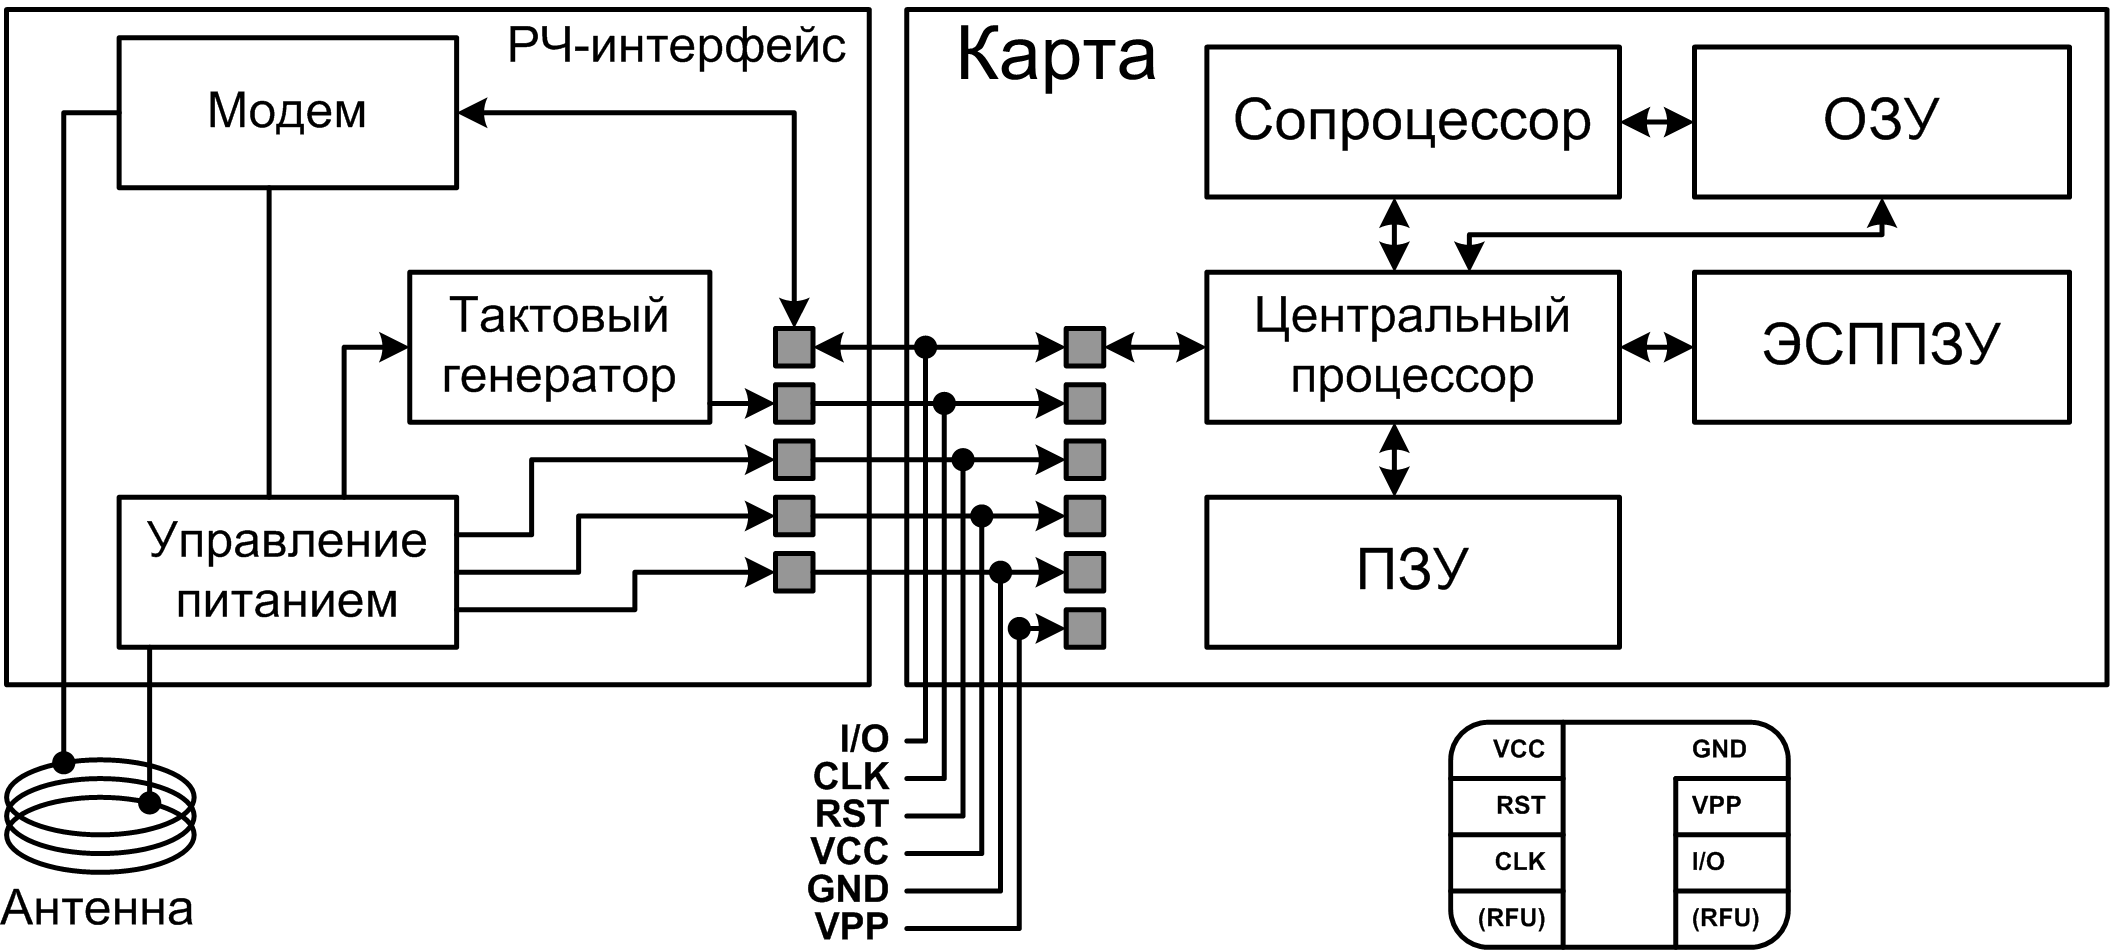
\includegraphics[width=.9\textwidth]{pict/chipcard} }
            \mode<article>{ 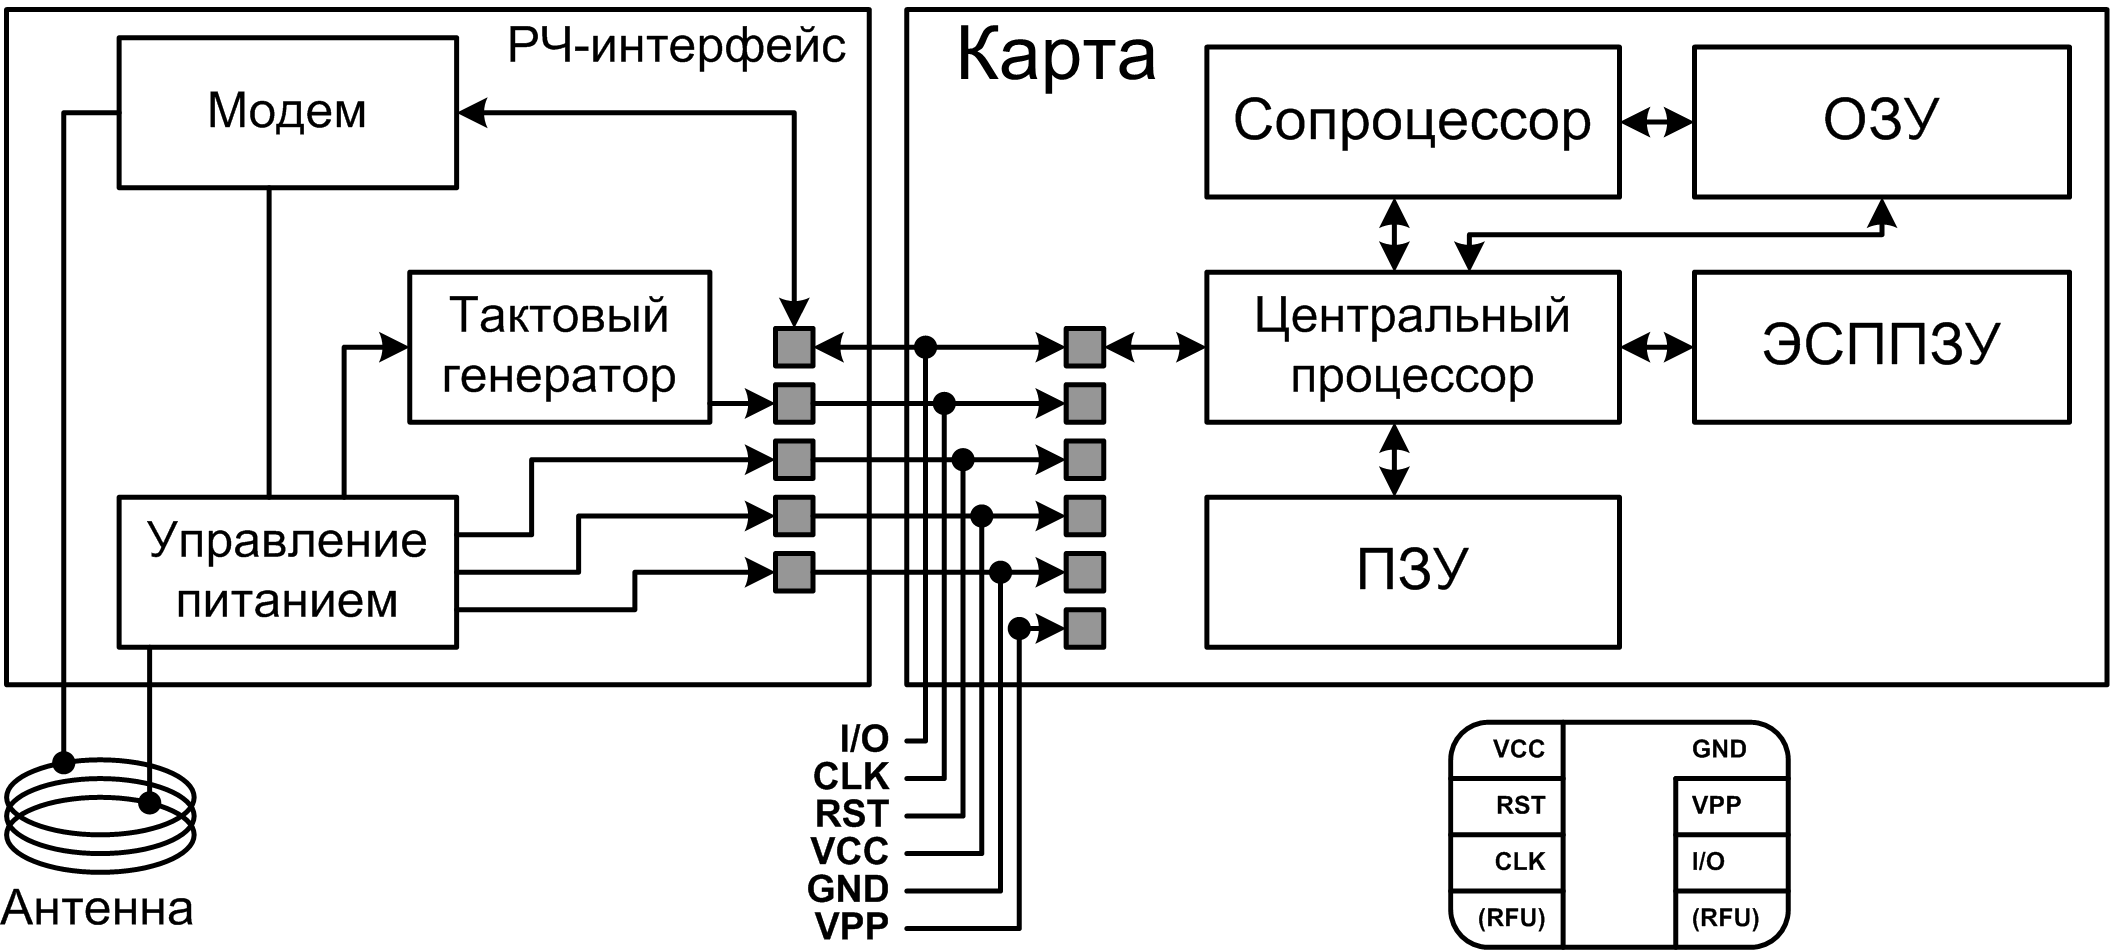
\includegraphics[width=.7\textwidth]{pict/chipcard} } 
            \caption{Архитектура чип-карты}\label{pict:chipcard}
        \end{center}
    \end{figure} 
    
    \mode<article>{см. Рис. \ref{pict:chipcard}}
\end{frame}


\begin{frame}
    \frametitle{Чип-карты}
    \framesubtitle{Операционная система карты. ISO/IEC 7816-4}
    Задачи.
    \begin{itemize}
        \item Управление передачей данных к смарт-карте и от нее.
        \item Реализация монитора обращений.
        \item Управление исполнением команд.
        \item Организация файловой системы и управление файлами.
        \item Криптографические функции.
        \item Установка и загрузка прикладных программ. 
            \mode<article>{
                Примером может служить Java Card. Расширение функционалных возможностей карты за счет
                прикладных программ --- дополнительные проблемы безопасности.
            }
    \end{itemize}
\end{frame}

\begin{frame}
    \frametitle{Чип-карты}
    \framesubtitle{Файловая система. ISO/IEC 7816-4(5)}
    
    \begin{figure}
        \begin{center}
            \mode<presentation>{ 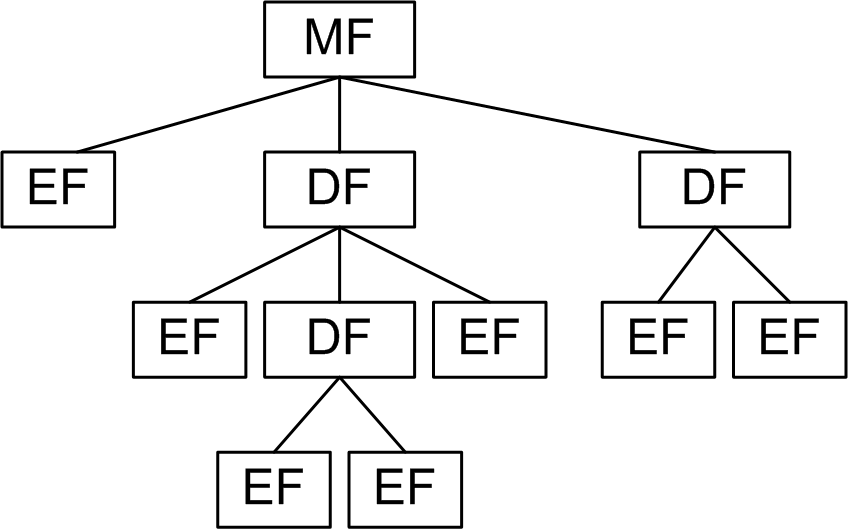
\includegraphics[width=.8\textwidth]{pict/cardmem} }
            \mode<article>{ 
                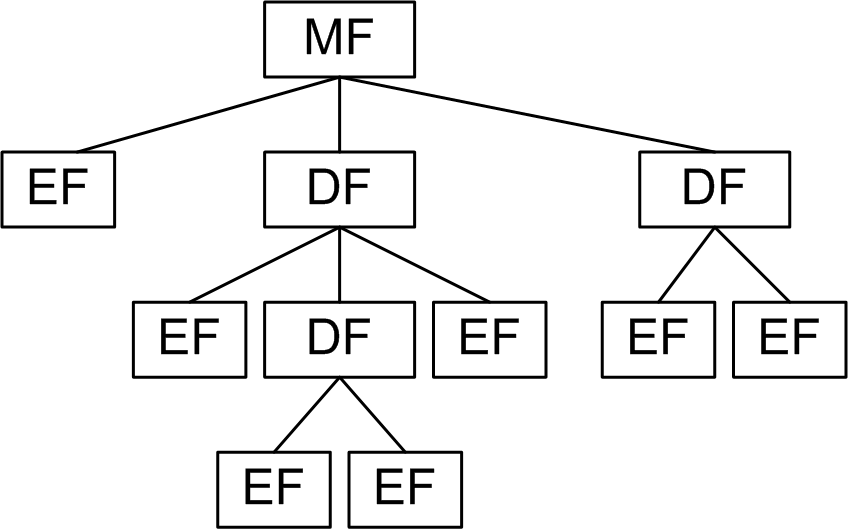
\includegraphics[width=.7\textwidth]{pict/cardmem}
                \caption{Архитектура чип-карты}\label{pict:cardmem}
            }
        \end{center}
    \end{figure} 
    
    \mode<article>{см. Рис. \ref{pict:cardmem}}
\end{frame}


\begin{frame}
    \frametitle{Чип-карты}
    \framesubtitle{Файловая система. ISO/IEC 7816-4(5)}
    Структура.
    \begin{enumerate}
        \item MF (Master File) --- главный файл (каталог). 
            \mode<article>{Содержит DF и EF. Существует в единственном экземпляре.}
        \item DF (Dedicated File) --- файл каталога. 
            \mode<article>{Содержит DF и EF. На картах вложенность каталогово обычно не превышает 2}
        \item EF (Elementary File) --- элементарный файл. 
            \mode<article>{Содержит данные.}
    \end{enumerate}
    Типы EF (элементарных файлов).
    \begin{itemize}
        \item Простой двоичный файл.
        \item Линейный файл с записями фиксированной или переменной длины.
            \mode<article>{Доступ к записям может осуществляться последовательно или по смещению записи от начала.}
        \item Циклический файл с записями фиксированной длины.
            \mode<article>{Логика работы с циклическим списком.}
    \end{itemize}
\end{frame}


\begin{frame}
    \frametitle{Чип-карты}
    \framesubtitle{Java Card}
    
    \begin{itemize}
        \item Отраслевой стандарт.
        \item Ограниченная реализация виртуальной Java машины.
        \item На данный момент используется версия 3.
        \item Развитый фреймворк для разработки прикладных решений.
        \begin{itemize}
            \item Возможность <<прозрачной>> работа с файловой системой.
            \item Обмен данными с терминалом в рамках ISO/IEC 7816-4.
            \item Криптографические функции.
        \end{itemize}
        \item Безопасная загрузка апплетов в виде CAP-файлов.
    \end{itemize}
\end{frame}


\begin{frame}
    \frametitle{Чип-карты}
    \framesubtitle{Java Card. Компоненты Java Card}
    
    \begin{figure}
        \begin{center}
            \mode<presentation>{ 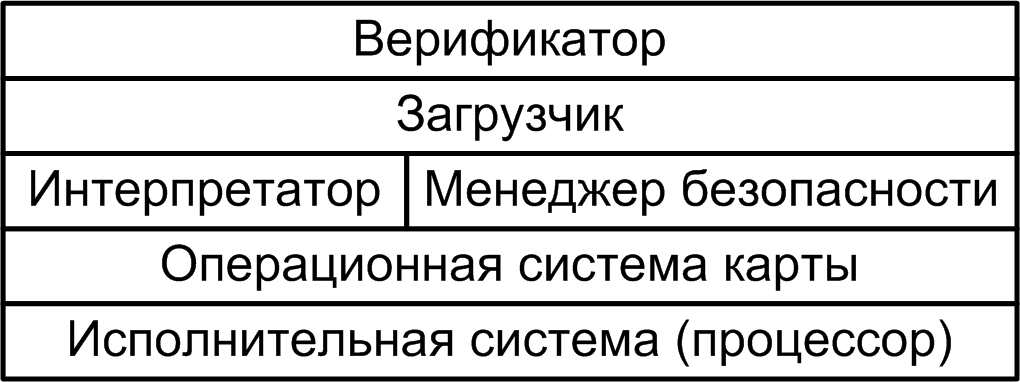
\includegraphics[width=.9\textwidth]{pict/jcardcomp} }
            \mode<article>{ 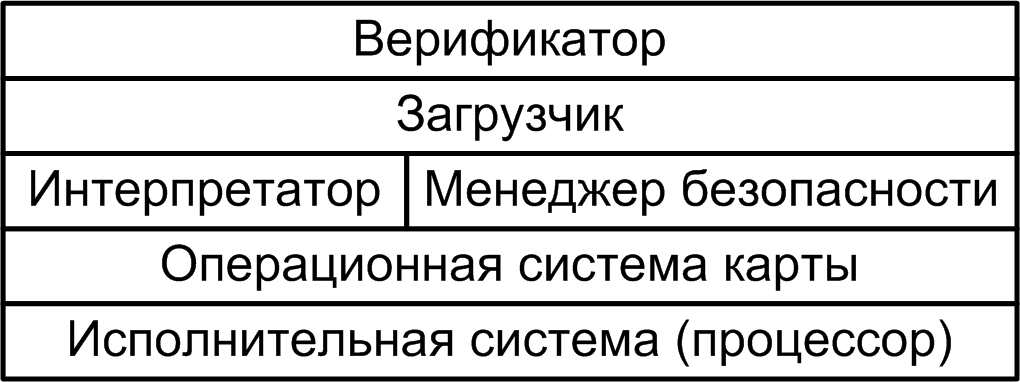
\includegraphics[width=.7\textwidth]{pict/jcardcomp} } 
            \caption{Компоненты Java Card}\label{pict:jcardcomp}
        \end{center}
    \end{figure} 
    
    \mode<article>{см. Рис. \ref{pict:jcardcomp}}
\end{frame}


\begin{frame}
    \frametitle{Чип-карты}
    \framesubtitle{Java Card. Структура программного обеспечения}
    
    \begin{figure}
        \begin{center}
            \mode<presentation>{ 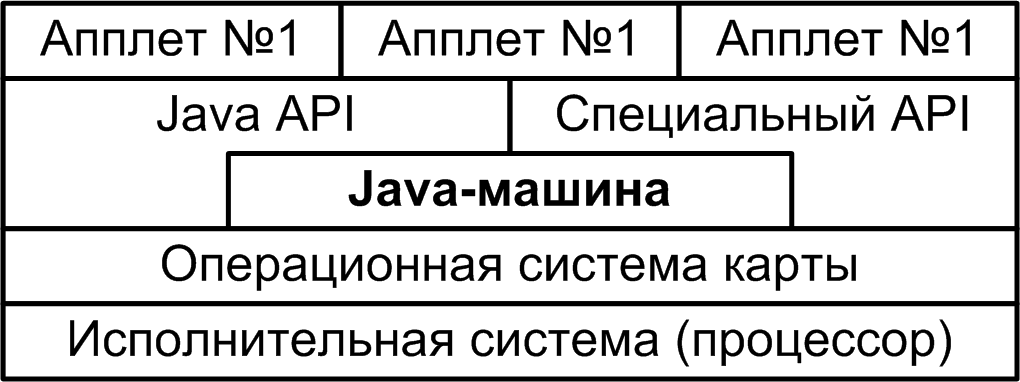
\includegraphics[width=.9\textwidth]{pict/jcardsoft} }
            \mode<article>{ 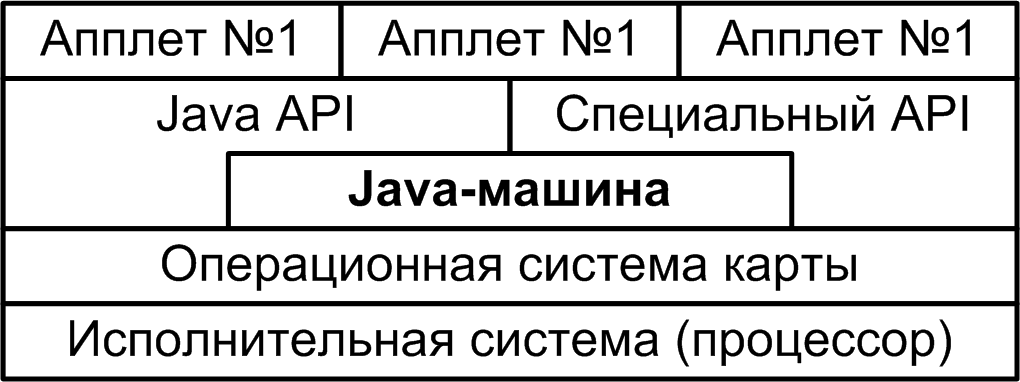
\includegraphics[width=.7\textwidth]{pict/jcardsoft} } 
            \caption{Структура программного обеспечения}\label{pict:jcardsoft}
        \end{center}
    \end{figure} 
    
    \mode<article>{см. Рис. \ref{pict:jcardsoft}}
\end{frame}


\begin{frame}
    \frametitle{Чип-карты}
    \framesubtitle{Стандарты}
    
    \begin{itemize}
        \item \alert{ISO/IEC 7816} --- базовый стандарт.
        \begin{itemize}
            \item Определяет физические параметры карт, 
            расположение контактов, электрические параметры. 4-я часть определяет протокол обмена 
            и механизм действия команд. Остальные части расширяют и уточняют 4-ю часть.
        \end{itemize}
        
        \item \alert{ISO/IEC 10536} --- стандарт для бесконтактных карт поверхностного действия.
        
        \item \alert{ISO/IEC 14443} --- стандарт для бесконтактных пассивных карт (Proximity cards) ближнего радиуса действия (до 10 см).
        
        \item \alert{ISO/IEC 15693} --- стандарт для бесконтактных пассивных карт (Vicinity cards) дальнего радиуса действия (более 10 см).
        
    \end{itemize}
\end{frame}



\subsection{USB-ключи}


\begin{frame}
    \frametitle{USB-ключи}
    \framesubtitle{Внешний вид}
    
    \begin{figure}
        \begin{center}
            \mode<presentation>{ 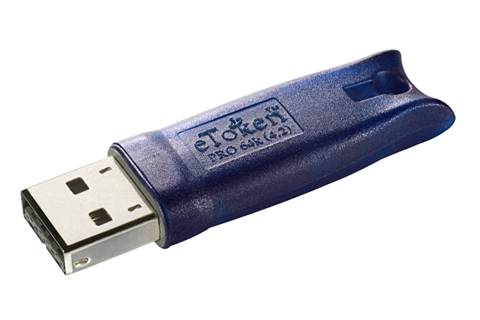
\includegraphics[width=.4\textwidth]{pict/etoken} }
            \mode<article>{ 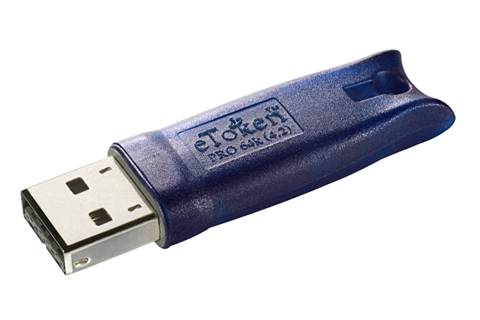
\includegraphics[width=.4\textwidth]{pict/etoken} } 
            \caption{USB-ключ eToken}\label{pict:etoken}
        \end{center}
    \end{figure} 
    
    \mode<article>{см. Рис. \ref{pict:etoken}}
\end{frame}


\begin{frame}
    \frametitle{USB-ключи}
    \framesubtitle{Области применения}
    
    \begin{itemize}
        \item Контроль доступа к компьютеру.
        \item Криптографическая защита.
        \begin{itemize}
            \item Реализация DES, 3-DES, RC2, RC4, RC5, SHA-1, MD5, RSA, ГОСТ 28147-89 и т.д.
        \end{itemize} 
        \item Защищенное хранение данных.
        \item Аутетнификация и защита программ и данных. Например.
        \begin{itemize}
            \item Управление жизненным циклом ПО.
            \item Защита от нелегального: копирования, использования и распространения.
        \end{itemize} 
    \end{itemize} 
\end{frame}


\begin{frame}
\frametitle{USB-ключи}
\framesubtitle{Особенности}
\begin{itemize}
    \item Архитектурный аналог чип-карт (меньше требований к размерам микрочипа).
    \item Не требуют специальных адаптеров для подключения к компьютеру.
    \item Используются в гибридной схеме совместно с RFID.
\end{itemize}
\end{frame}


\appendix %приложения


\begin{frame}
    \frametitle{Источники}
    Обзор технолоний аппаратно-программной аутентификации можно найти в \cite{bib:shangin:protect,bib:djhuian:eid}.

    Подробнее ознакомиться с iButton можно на ресурсе \cite{bib:misc:ibutton}.

    Подробности об использовании USB-ключей, технологиями HASP, eToken можно на ресурсе \cite{bib:misc:aladdin}.

    Узнать больше о Java Card, скачать фреймворк и среды разработки можно на ресурсе \cite{bib:misc:oracle}.
\end{frame}


\begin{frame}[allowframebreaks]{Библиография}
    \bibliographystyle{gost780u}
    \bibliography{./../bibliobase}
\end{frame}

\end{document}